\documentclass[10pt,twocolumn,letterpaper]{article}
% IEEE conference layout built on the article class (IEEEtran.cls was not available
% in the build environment). Margins, fonts, heading and reference styles follow the
% IEEE conference template; the text can be pasted into IEEEtran unchanged.
\usepackage[T1]{fontenc}
\usepackage{mathptmx}
\usepackage[letterpaper,top=0.75in,bottom=1in,left=0.625in,right=0.625in,columnsep=0.25in]{geometry}
\usepackage{graphicx,booktabs,amsmath,cite,stfloats,balance,array}
\usepackage[hidelinks]{hyperref}
\usepackage[font=footnotesize,labelsep=period,justification=justified,singlelinecheck=false]{caption}
\usepackage{titlesec}
\renewcommand{\thesection}{\Roman{section}}
\renewcommand{\thesubsection}{\Alph{subsection}}
\titleformat{\section}{\centering\scshape\normalsize}{\thesection.}{0.5em}{}
\titlespacing*{\section}{0pt}{8pt}{4pt}
\titleformat{\subsection}{\itshape\normalsize}{\thesubsection.}{0.5em}{}
\titlespacing*{\subsection}{0pt}{6pt}{3pt}
\renewcommand{\figurename}{Fig.}
\renewcommand{\thetable}{\Roman{table}}
\captionsetup[table]{labelsep=newline,justification=centering,textfont=sc,font=footnotesize}
\setlength{\parindent}{1em}
\renewcommand\refname{References}
\makeatletter
\renewcommand\@biblabel[1]{[#1]}
\makeatother
\pagestyle{empty}

\begin{document}
\twocolumn[{%
\begin{center}
{\fontsize{22}{26}\selectfont Testing Land Cover and Population as Drivers of River Total Dissolved Solids in a Data-Scarce Tropical Basin: A Routed Model with Independent Validation for the Mindanao River Basin, Philippines\par}
\vspace{12pt}
\begin{tabular}{c@{\hspace{40pt}}c}
\normalsize Peter Dominic C. Montero & \normalsize Jay M. Navaluna\textsuperscript{*} \\
\footnotesize\itshape Department of Civil Engineering & \footnotesize\itshape Department of Civil Engineering \\
\footnotesize\itshape University of Southern Mindanao & \footnotesize\itshape University of Southern Mindanao \\
\footnotesize\itshape Kabacan, Cotabato 9407, Philippines & \footnotesize\itshape Kabacan, Cotabato 9407, Philippines \\
\footnotesize s.pdcmontero@usm.edu.ph & \footnotesize jmnavaluna@usm.edu.ph \\
\footnotesize ORCID 0009-0004-6553-6348 & \footnotesize ORCID 0000-0001-8889-0527
\end{tabular}
\vspace{14pt}
\end{center}}]
{\let\thefootnote\relax\footnotetext{\textsuperscript{*}Corresponding author.}}

\noindent\textbf{\textit{Abstract}---GIS indices that screen river water quality in data-scarce basins are seldom tested against observations. We built a routed mass-balance model of total dissolved solids (TDS) for the Mindanao River Basin (20,583~km$^2$) from open data---the ALOS AW3D30 elevation model, ESA WorldCover 2021 land cover and WorldPop 2020 population (5.16 million people)---and tested it against every georeferenced published TDS value we could find: 22 sites on 7 river systems. The model routes runoff, land-cover solute loads and population loads down a 90~m D8 network in MATLAB-compatible code (run in GNU Octave). Five model structures were fitted by non-negative least squares and tested on six independent literature sites, by leave-one-site-out and by leave-one-river-out cross-validation, with 2000 bootstrap refits and a 200-draw Monte Carlo on runoff coefficients. No structure predicted held-out sites better than the training mean: leave-one-river-out RMSE was 54.1~mg/L for the best structure (a uniform land background plus a population term) against 52.5~mg/L for the null model, and all structures under-predicted the independent sites by 45--68~mg/L, most strongly on the volcanic slopes of Mt Apo (observed 300~mg/L, predicted 107--116~mg/L). The population term was positive in three of the four structures that included it, and raising population by 50\% raised simulated outlet TDS by 7.3~mg/L (95\% interval 0.0--29.6), whereas the simulated effect of converting forest to cropland ranged from $-1.0$ to $-23.5$~mg/L across structures because no structure could identify a cropland source. Published data therefore cannot resolve land-cover effects on TDS in this basin; between-river differences, probably geological, dominate. We release the model, data and 3D visualisations, and propose a 30-site sampling network to supply the missing evidence.}

\vspace{4pt}
\noindent\textbf{\textit{Index Terms}---total dissolved solids, flow routing, land cover, population, mass balance, cross-validation, Monte Carlo, Mindanao River Basin, MATLAB.}

\section{Introduction}
Total dissolved solids (TDS) measure the salts and small amounts of organic matter dissolved in water and are a standard indicator of salinity and general water-quality condition. River TDS reflects rock weathering, soils and residence time as well as inputs from farms, settlements and industry, so it varies with both the physical setting and the land use of a catchment \cite{asnake,merriam}. Where monitoring is dense, TDS can be mapped with geostatistical or machine-learning models trained on many observations \cite{stephens,aju}. Most tropical basins in the Philippines lack such data.

In data-scarce settings, GIS multicriteria evaluation is a common substitute: spatial factors are scored and combined by weighted overlay into a ``potential'' index \cite{malcz}. The weights encode judgement rather than evidence. Sensitivity analysis shows how much an index depends on them \cite{chen,ligmann} but not whether the index reflects observed conditions. An earlier version of this study built such an index for the Mindanao River Basin (MRB) from slope, flow accumulation and drainage density; reviewers rightly asked for a defensible weighting basis and validation against observed TDS.

Process-based alternatives exist. Export-coefficient and SPARROW-type models give each land-use class a characteristic contribution and route the loads through the river network \cite{johnes,sparrow}, and land-cover effects on water quality are known to vary between watersheds \cite{tu}. Because TDS is close to conservative in channels, a routed mixing model is physically reasonable and has few parameters, which a small set of observations can estimate---or reject.

The MRB is the largest basin in Mindanao \cite{guiamel}, yet basin-wide TDS information is fragmentary. This study asks whether the published TDS record supports GIS-based prediction of TDS from land cover and population. We (1) compile every georeferenced published TDS value in the basin and hold out an independent subset; (2) build a routed land-cover and population model in MATLAB-compatible code; (3) compare five model structures against a null model by independent testing and two forms of cross-validation; (4) propagate parameter and runoff-coefficient uncertainty; (5) simulate forest, farm, built-up and population scenarios and visualise them in 3D; and (6) design a sampling network that targets what the data cannot yet resolve.

\section{Materials and Methods}
\subsection{Workflow, Study Area and Open Data}
Fig.~\ref{fig:workflow} summarises the workflow. The MRB drains central Mindanao through the Pulangi River from the Bukidnon highlands and the Allah River from the South Cotabato highlands, which meet in the Liguasan Marsh before discharging to Illana Bay at Cotabato City \cite{guiamel}.

Elevation came from the ALOS World 3D--30~m (AW3D30) model \cite{tadono}, obtained from OpenTopography, reprojected to UTM Zone~51N and averaged to 90~m. Sea cells connected to the tile edge were masked, OpenStreetMap river lines were burned 20~m into the surface, depressions were filled \cite{wang}, flats were resolved and D8 directions computed \cite{ocallaghan}. Interior marsh sinks within 15~km of the network were linked to it. The delineated basin covers 20,583~km$^2$ (2.54 million cells), close to the 21,503~km$^2$ reported for the MRB \cite{guiamel}.

Land cover came from ESA WorldCover 2021 v200 at 10~m \cite{zanaga}, grouped into tree cover (64.8\% of the basin; includes tree plantations), cropland (14.7\%), built-up (1.0\%), grass/shrub/bare (16.8\%) and water/wetland (2.6\%), stored as fractions per 90~m cell. Population came from WorldPop 2020 at 1~km (unconstrained, UN-unadjusted) \cite{worldpop}, redistributed to 90~m cells by area; the basin holds 5.16 million people (Fig.~\ref{fig:area}).

\begin{figure*}[!t]
\centering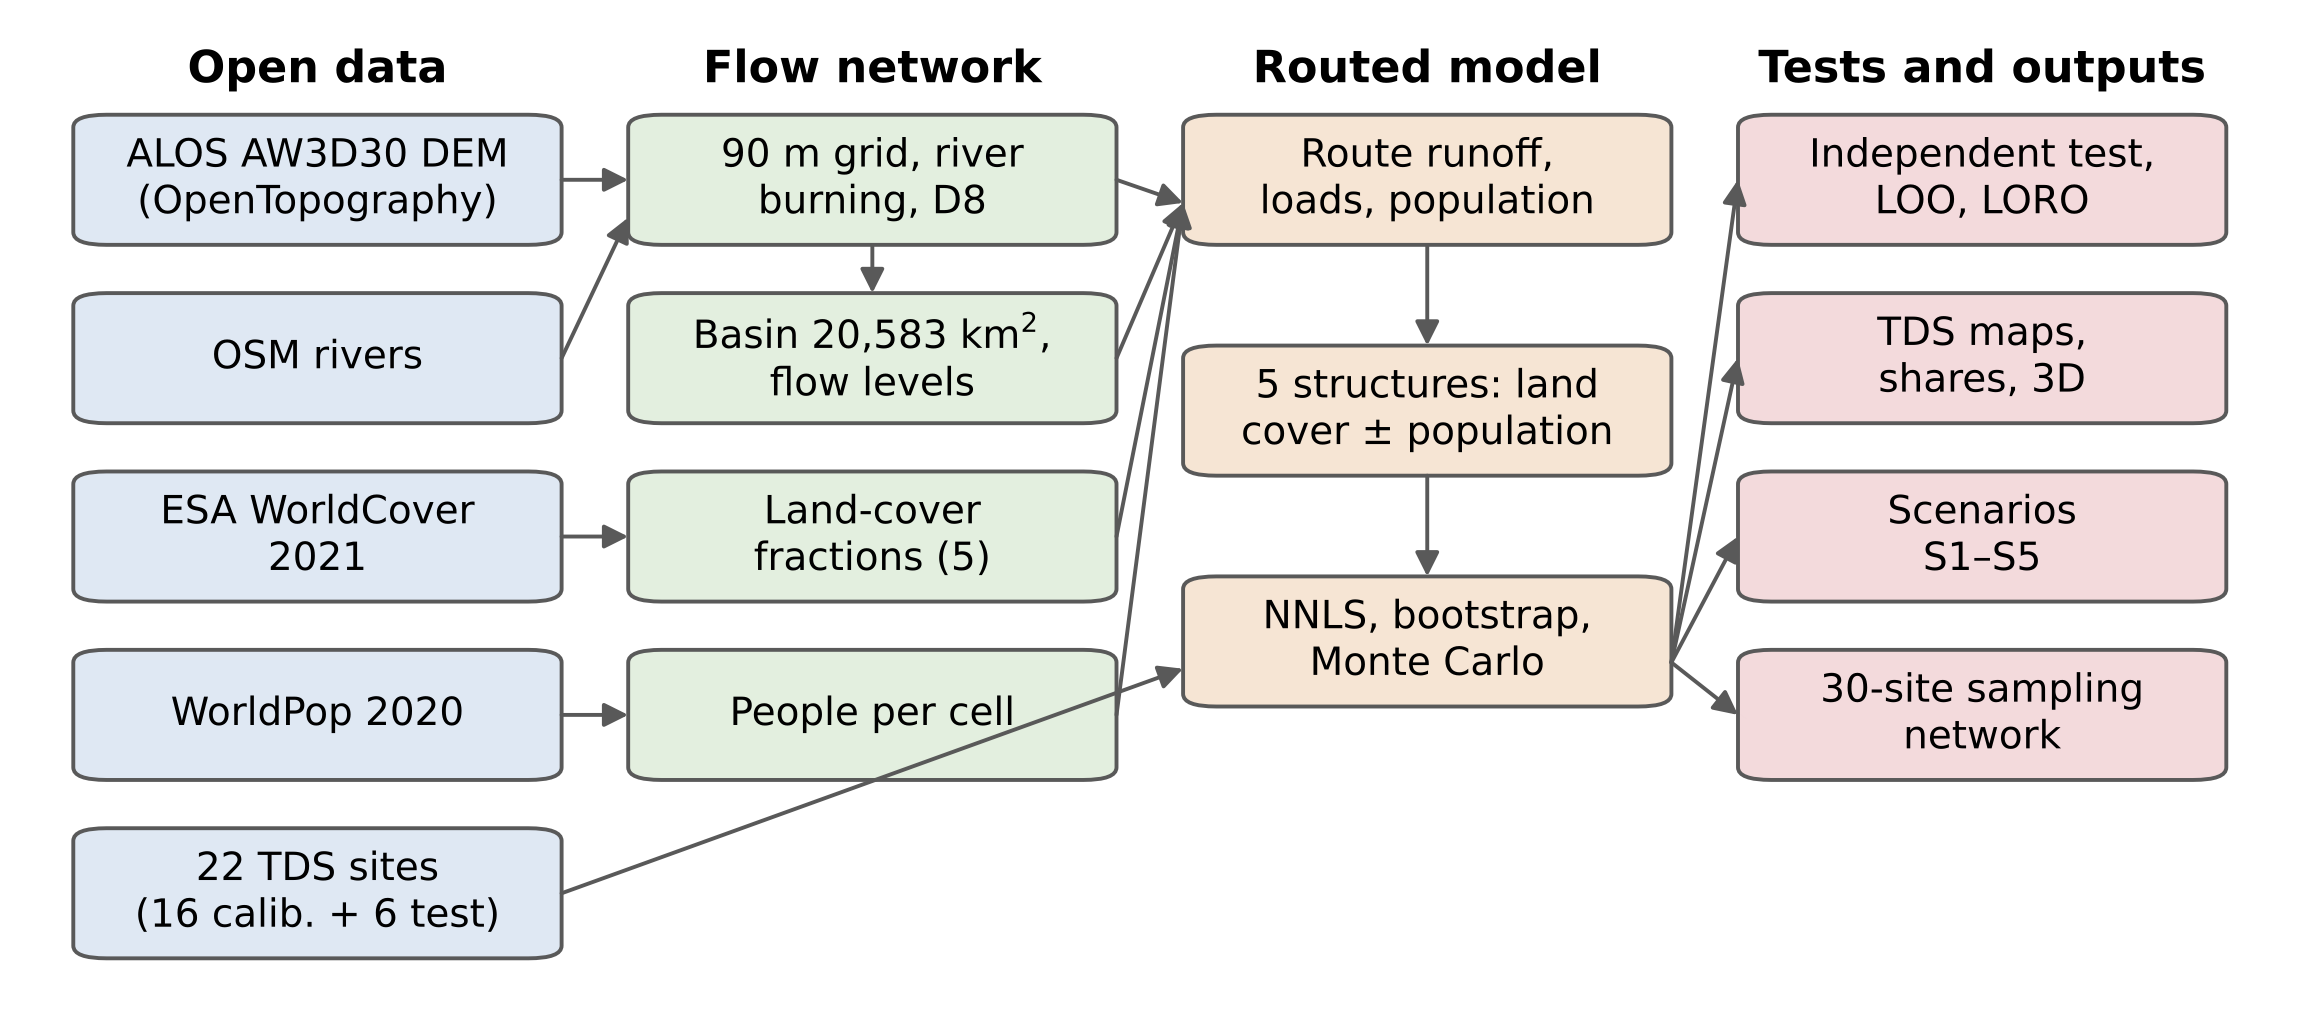
\includegraphics[width=0.86\textwidth]{fig1_workflow.png}
\caption{Workflow from open datasets through the 90~m flow network to the routed model, its tests against observed TDS, and its outputs. LOO, leave-one-site-out; LORO, leave-one-river-out.}
\label{fig:workflow}
\end{figure*}

\begin{figure*}[!t]
\centering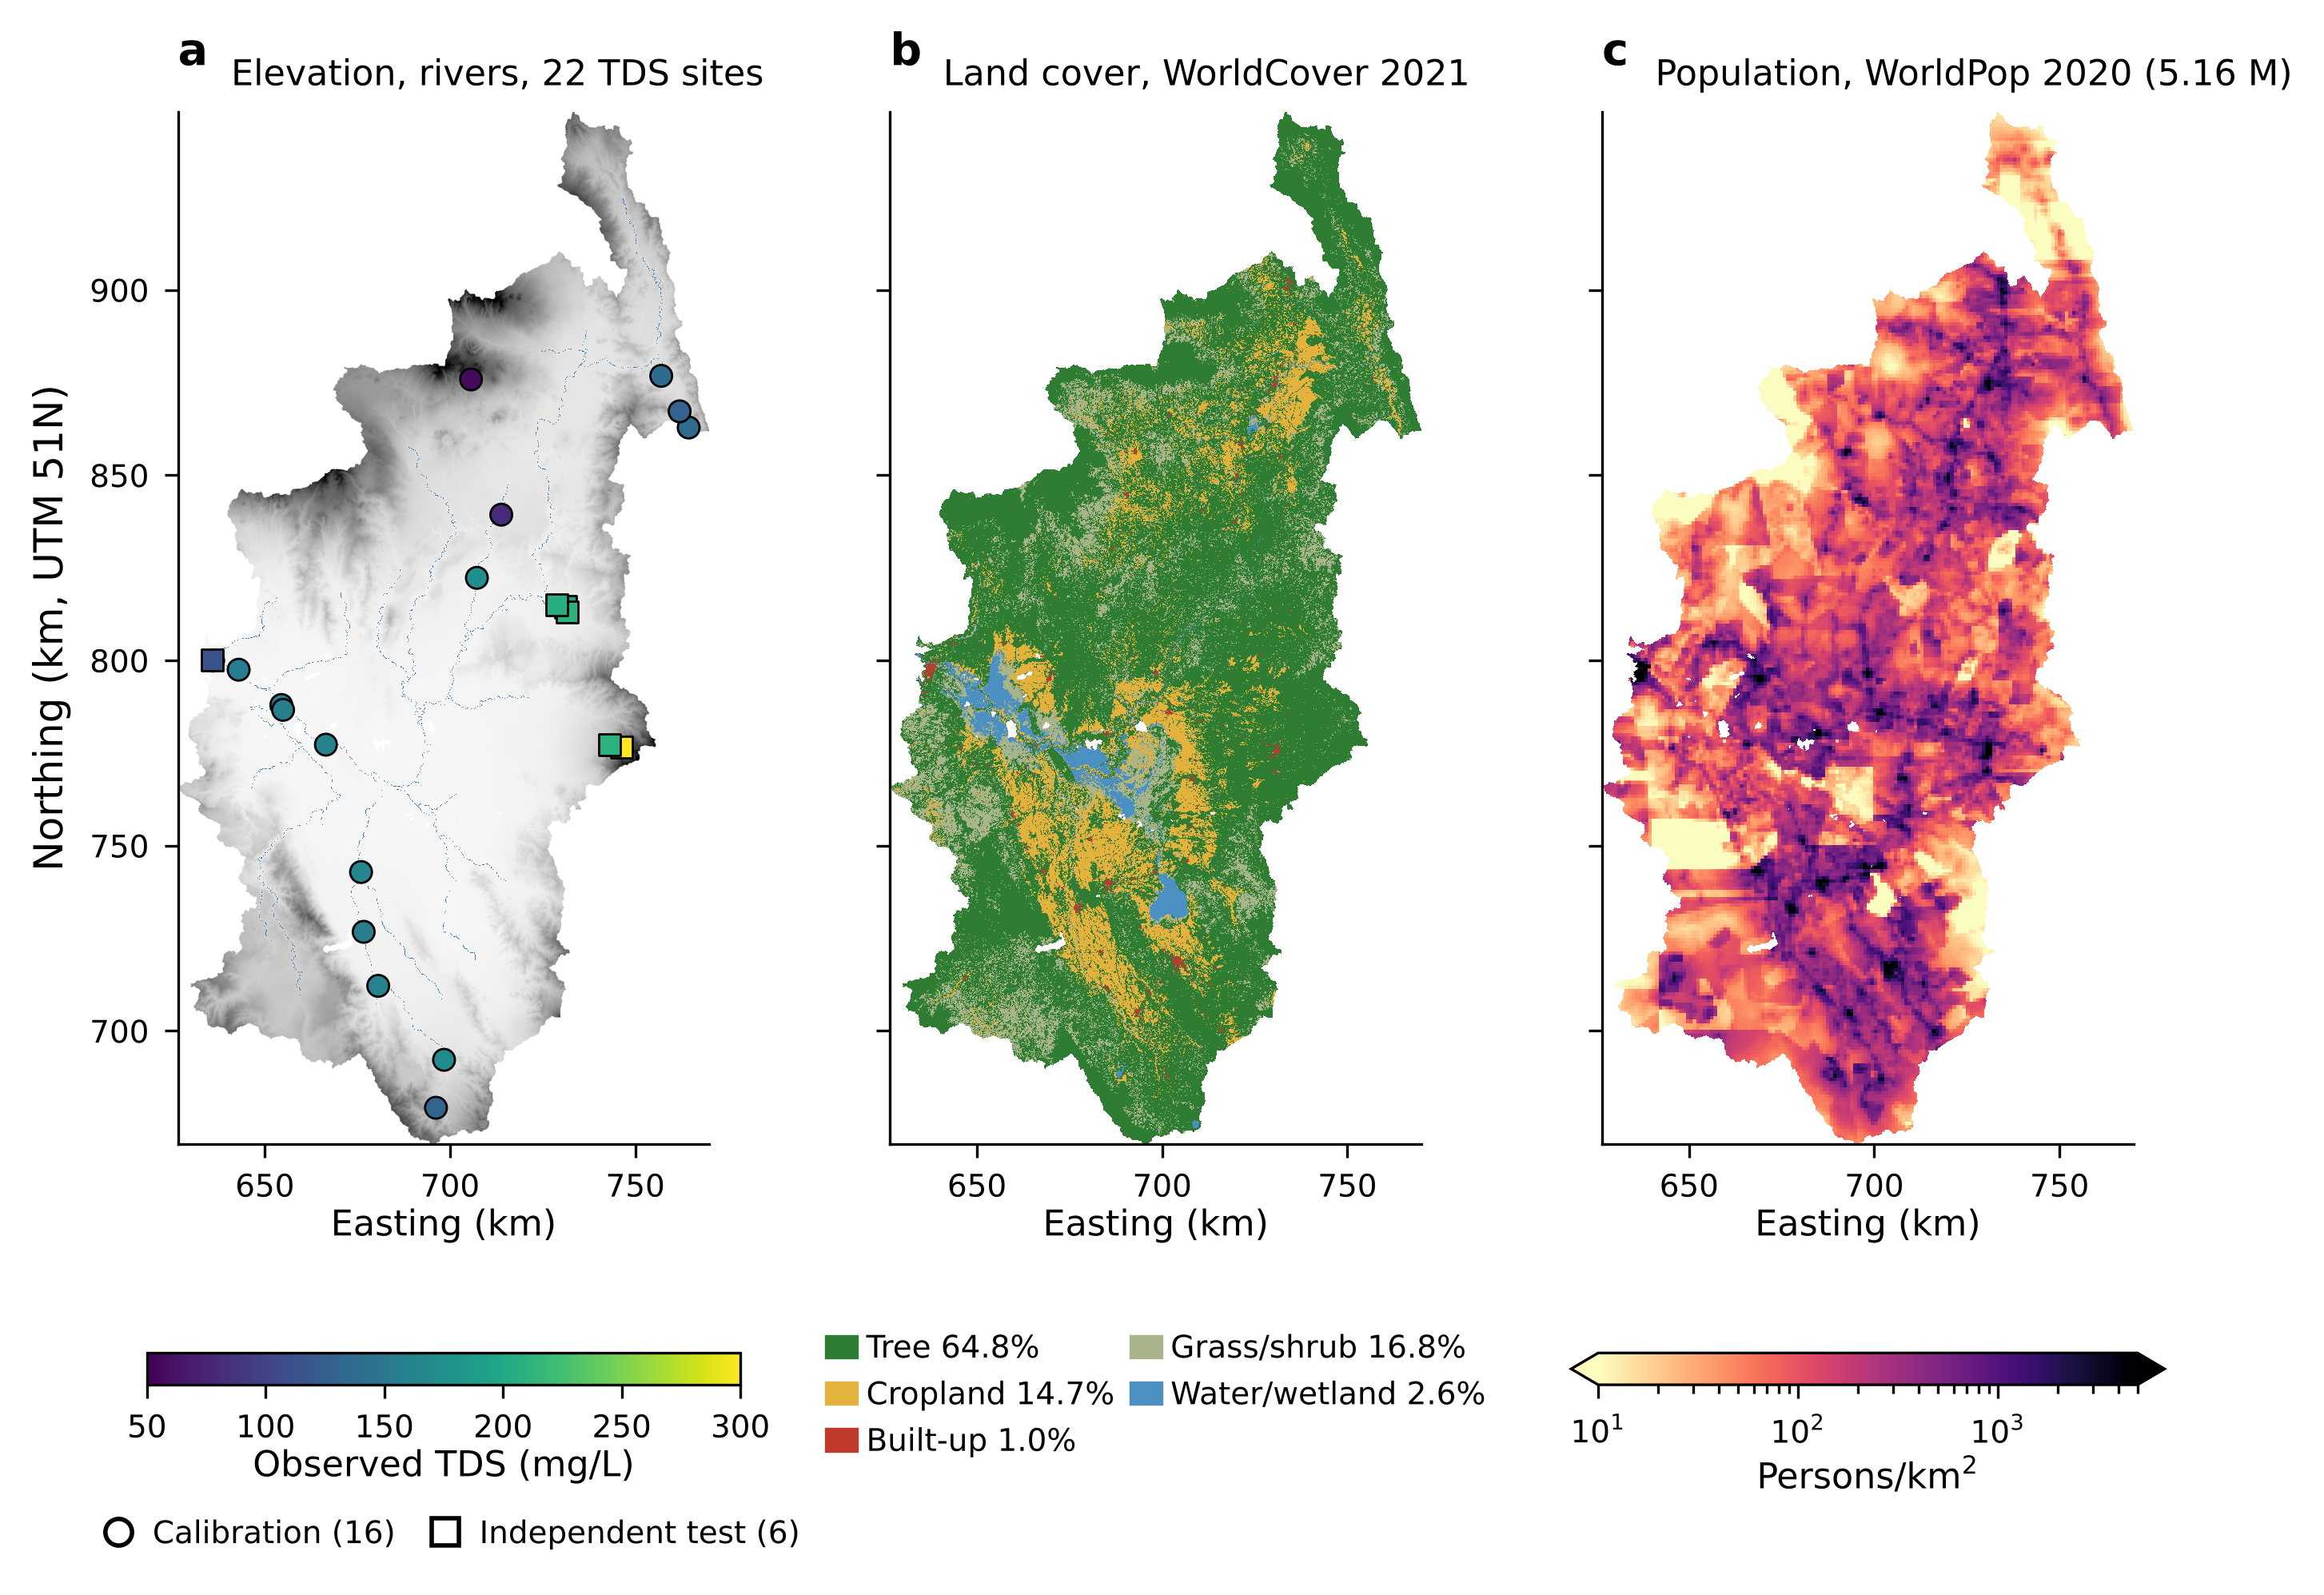
\includegraphics[width=\textwidth]{fig2_study_area.png}
\caption{Study area. (a) Delineated Mindanao River Basin on AW3D30 elevation, with channels draining $\geq$300~km$^2$ and the 22 published TDS sites coloured by observed TDS (circles, calibration; squares, independent test). (b) Dominant ESA WorldCover 2021 class per 90~m cell, with basin shares. (c) WorldPop 2020 population density. Coordinates are UTM Zone 51N.}
\label{fig:area}
\end{figure*}

\subsection{Observed TDS and the Independent Test Set}
We compiled every published TDS or electrical-conductivity value with site coordinates that we could find for rivers in the basin (Table~\ref{tab:obs}). Sixteen sites from four sources (2017--2024) formed the calibration set used in the first version of this study \cite{brillantes,dimalen,dumago,galarpe}. Rio Grande conductivity \cite{dimalen} was converted to TDS with the TDS/EC ratio (0.504) of the Allah River surveys, which report both \cite{brillantes}; one Salug River point drains outside the basin and was excluded. Six further sites were found later and kept aside as an independent test: three on the Kulaman and Tinanan rivers in the Arakan Valley (five-month laboratory means, 2009--2010) \cite{villabeto}, two on the Marbel and Matingao rivers on Mt Apo (2012--2015) \cite{quimpang}, and one Rio Grande value at Cotabato City (August 2022) \cite{alombro}. The Mt Apo values were reported without units and were read as g/L (0.25--0.35 and 0.16--0.26); the Arakan site positions were inferred from the published description; and the Cotabato City value is the mean of three stations at an approximate location. Each point was snapped to the highest-accumulation cell within 270~m. The 22 sites span 2009--2024, mixed seasons and instruments, and 7 river systems.

\begin{table}[!t]
\caption{Published TDS Observations Used (n = 22)}
\label{tab:obs}
\centering\footnotesize
\setlength{\tabcolsep}{3pt}
\begin{tabular}{@{}lcccc@{}}
\toprule
River system (source) & Sites & Period & TDS (mg/L) & Area (km$^2$)\\
\midrule
\multicolumn{5}{@{}l}{\textit{Calibration}}\\
Allah River \cite{brillantes} & 5 & 2024 & 130--170 & 87--1930\\
Rio Grande de Mindanao \cite{dimalen} & 5 & 2024 & 155--166$^a$ & 15,722--20,577\\
Muleta watershed \cite{dumago} & 3 & 2017 & 57--173 & 6--734\\
Tigua River \cite{galarpe} & 3 & 2017 & 130--137 & 21--292\\
\multicolumn{5}{@{}l}{\textit{Independent test}}\\
Kulaman--Tinanan \cite{villabeto} & 3 & 2009--10 & 194--211 & 182--537\\
Mt Apo rivers \cite{quimpang} & 2 & 2012--15 & 210--300$^b$ & 7--16\\
Rio Grande, Cotabato City \cite{alombro} & 1 & 2022 & 114 & 20,577\\
\bottomrule
\end{tabular}\\[2pt]
\raggedright\scriptsize $^a$From EC with TDS/EC = 0.504. $^b$Reported without units; read as g/L.
\end{table}

\subsection{Routed Land-Cover and Population Model}
Each cell $i$ generates runoff in proportion to the area-weighted runoff coefficients $r_k$ of its land-cover fractions $f_{ik}$, solute load in proportion to that runoff times a class source concentration $c_k$, and a population load $\beta P_i$, where $P_i$ is its population in thousands. Runoff coefficients were set to mid-range rational-method values \cite{chow} (our choice): 0.20 tree cover, 0.35 cropland, 0.80 built-up, 0.30 grass/shrub/bare and 0.50 water/wetland. With uniform rainfall, which cancels from concentrations, water and loads are accumulated down the D8 network, and TDS at cell $j$ is
\begin{equation}
\mathrm{TDS}_j=\frac{\sum_k c_k\sum_{i\in U(j)} f_{ik}r_k+\beta\sum_{i\in U(j)}P_i}{\sum_{i\in U(j)}\sum_k f_{ik}r_k},
\label{eq:tds}
\end{equation}
where $U(j)$ is the set of cells upstream of and including $j$. TDS is treated as conservative in the channel \cite{johnes,sparrow}. Eq.~(\ref{eq:tds}) is linear in $c_k$ and $\beta$, which were estimated by non-negative least squares (NNLS) \cite{lawson}. Routing is vectorised by topological flow level, so one pass over 2.54 million cells takes a few seconds. The code (\texttt{tds\_route.m}, \texttt{run\_tds\_model.m}, \texttt{scenario\_by\_structure.m}) needs no toolboxes and runs in MATLAB R2016b or later; the results reported here were produced by the same code in GNU Octave 10.3.0.

\subsection{Model Structures, Validation and Uncertainty}
Five structures were compared: tree/non-tree; tree/non-tree + population; tree/cropland/other + population; all five classes + population; and a uniform land background + population, in which land cover affects only how much water dilutes the loads. Each was scored three ways against a null model that predicts the training-set mean: (i) fitted on the 16 calibration sites and used to predict the 6 independent sites; (ii) leave-one-site-out (LOO) on all 22 sites; and (iii) leave-one-river-out (LORO), holding out each of the 7 river systems in turn because sites on one river are not independent \cite{roberts}. The structure with the lowest LORO error was selected. Its 95\% parameter intervals came from 2000 bootstrap refits to resampled sites \cite{efron}, and a 200-draw Monte Carlo varied every runoff coefficient uniformly within $\pm$50\% of its nominal value, refitting the model each time.

\subsection{Scenarios, Source Apportionment and 3D Visualisation}
Five scenarios were applied to every cell: S1, 20\% of tree cover converted to cropland; S2, built-up area doubled at the expense of cropland (then tree cover); S3, 20\% of cropland converted to tree cover; S4, population +50\%; and S5, S1 and S4 together. Outlet changes for the selected structure carry 95\% bootstrap intervals; because the selected structure cannot separate land-cover classes by design, every scenario was also run under all five structures, each refitted to the 22 sites. Simulated TDS, the population share and scenario changes were mapped and draped in 3D over the AW3D30 terrain (vertical exaggeration $\times$12).

\subsection{Sampling-Network Design}
Candidate sites were channel cells draining 10--300~km$^2$, thinned to a 1~km lattice and split into five strata of upstream tree-cover fraction. Six sites per stratum were chosen greedily to maximise distance from the published sites and from each other.

\section{Results}
\subsection{Validation: No Structure Beats the Null Model}
Adding classes and a population term did not improve prediction (Table~\ref{tab:cv}, Fig.~\ref{fig:val}a). The null model had the lowest error in all three tests: 50.2~mg/L by LOO, 52.5~mg/L by LORO and 82.5~mg/L on the independent test. The best model structure by LORO, uniform background + population, came within 1.6~mg/L of the null (54.1~mg/L) but had a negative Nash--Sutcliffe efficiency ($-0.28$). The tree/non-tree model that was selected in the first version of this study, on 16 sites, was the worst structure once the 22 sites were used (LORO 61.2~mg/L).

\begin{table}[!t]
\caption{Model Comparison (RMSE in mg/L; Bias = Mean Prediction Error)}
\label{tab:cv}
\centering\footnotesize
\setlength{\tabcolsep}{2.5pt}
\begin{tabular}{@{}lccccc@{}}
\toprule
Structure & $p$ & Test & Test bias & LOO & LORO\\
\midrule
Null (training mean) & 1 & 82.5 & $-62.4$ & 50.2 & 52.5\\
Tree / non-tree & 2 & 96.4 & $-68.2$ & 58.8 & 61.2\\
Tree / non-tree + pop. & 3 & 96.4 & $-61.7$ & 59.9 & 62.7\\
Tree / crop / other + pop. & 4 & 84.9 & $-44.9$ & 56.1 & 58.8\\
Five classes + pop. & 6 & 87.6 & $-49.7$ & 56.2 & 60.1\\
Uniform + pop. (selected) & 2 & 95.9 & $-62.3$ & 53.2 & 54.1\\
\bottomrule
\end{tabular}\\[2pt]
\raggedright\scriptsize $p$, parameters. Test: fitted on 16 calibration sites, predicting 6 independent sites. LOO and LORO use all 22 sites.
\end{table}

\begin{figure*}[!t]
\centering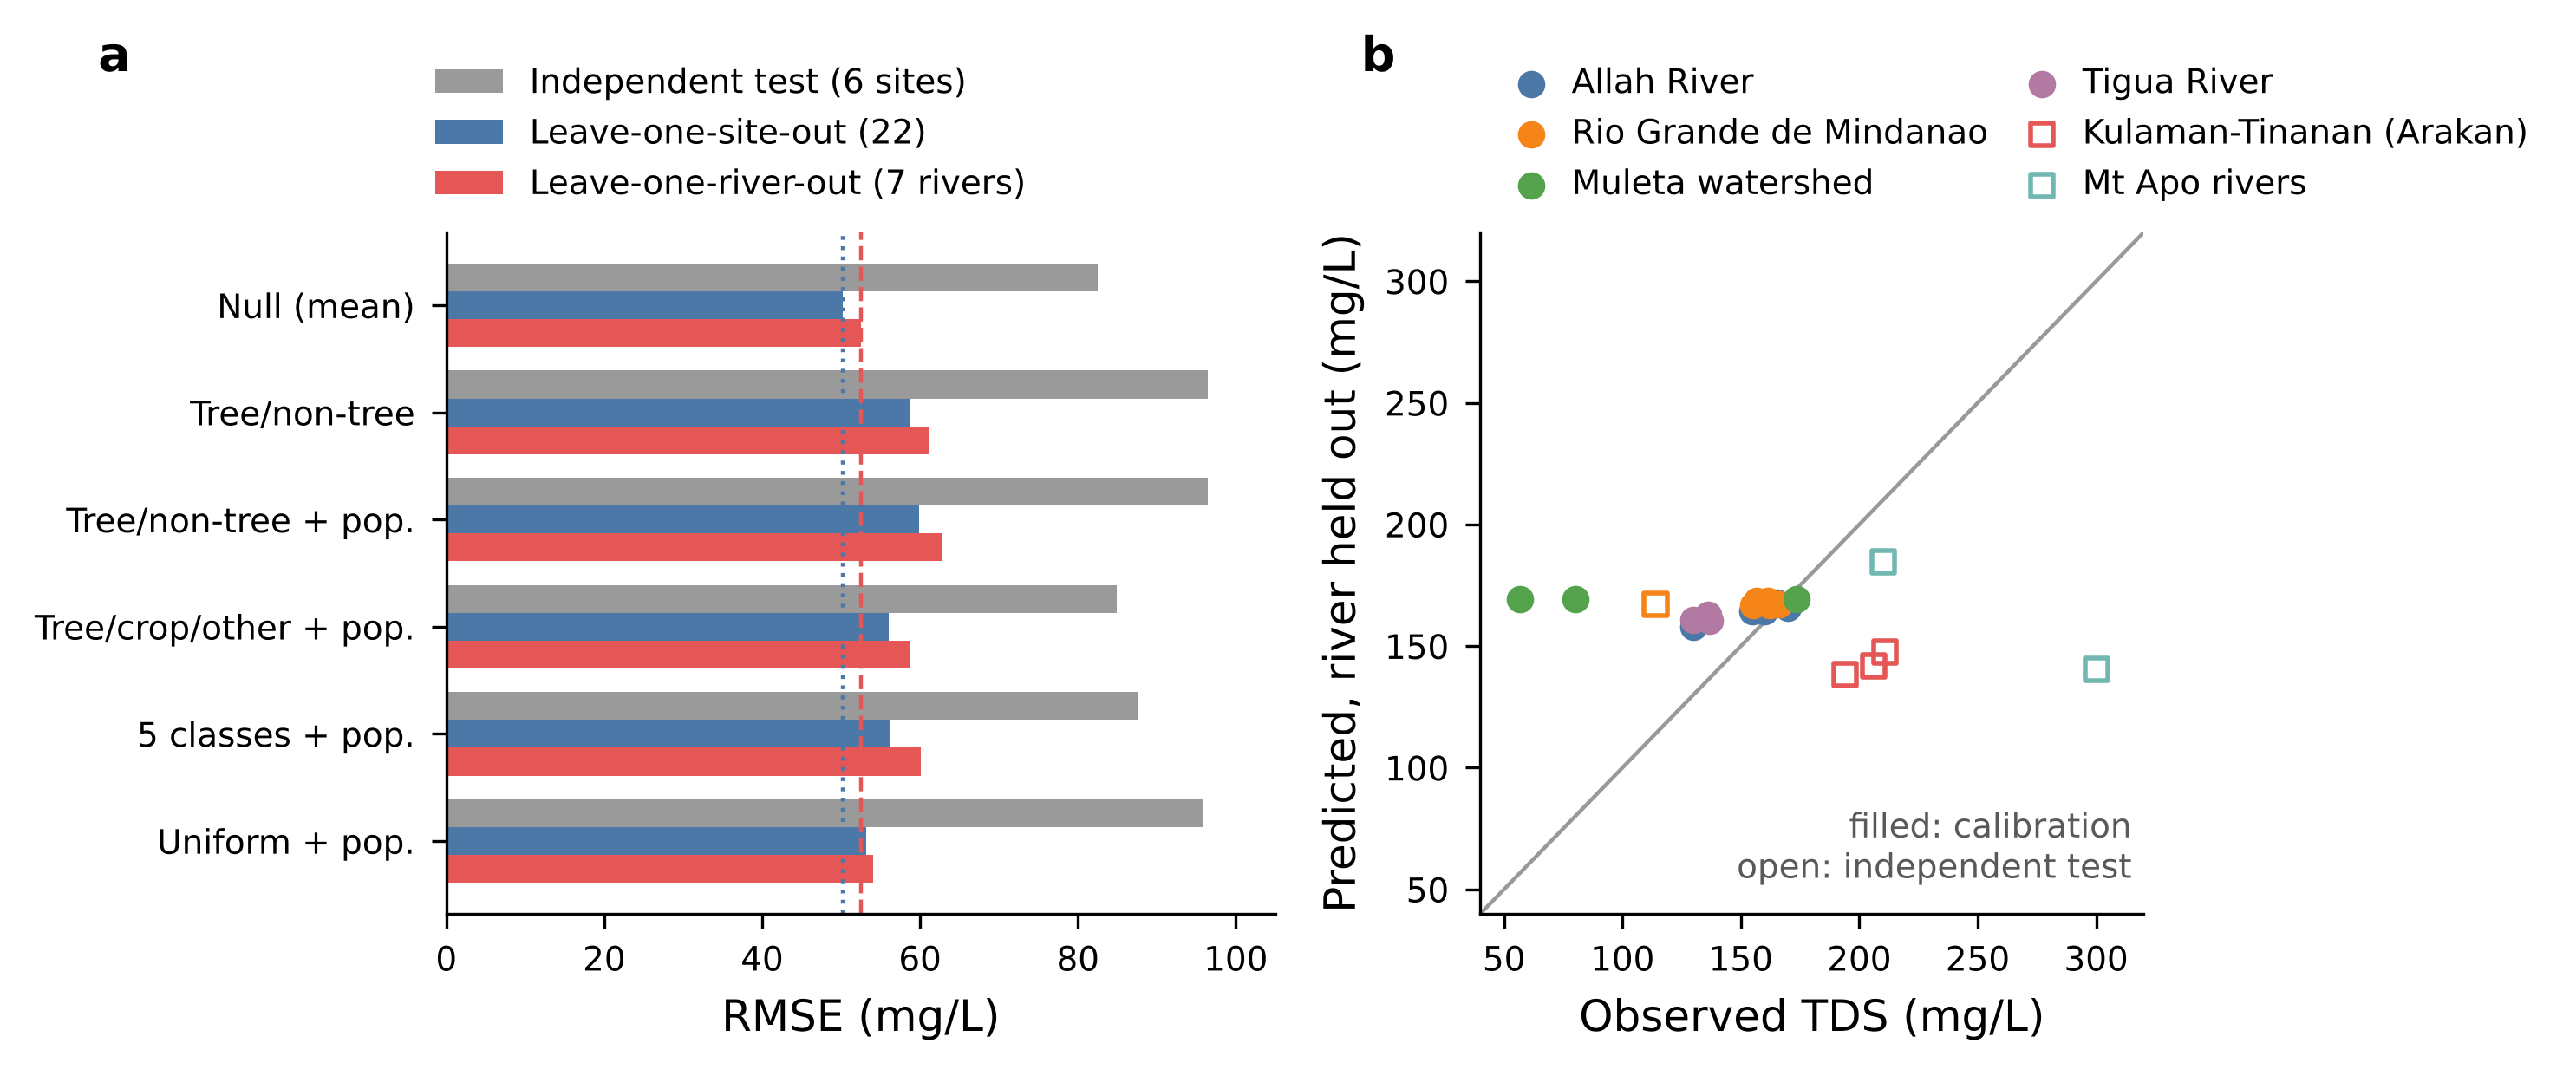
\includegraphics[width=\textwidth]{fig4_model_validation.png}
\caption{Model evaluation. (a) RMSE of each structure on the independent test, by LOO and by LORO; dotted and dashed lines mark the null model's LOO and LORO errors. (b) Observed TDS against LORO predictions of the selected structure (uniform background + population); the grey line is 1:1. Filled markers, calibration sites; open markers, independent sites.}
\label{fig:val}
\end{figure*}

The independent sites show why. Every structure under-predicted them, by 45--68~mg/L on average (Table~\ref{tab:cv}). The three Arakan Valley sites (194--211~mg/L) were predicted at 111--176~mg/L, and the Marbel River on Mt Apo (300~mg/L) at 107--116~mg/L, while the 2022 Cotabato City value (114~mg/L) was over-predicted (152--165~mg/L) and lies 41--52~mg/L below the 2024 survey at the same river \cite{dimalen}. Within the calibration set, the two lowest values, the Upper Baguik-ikan headwater (57~mg/L) and the Malinao River (80~mg/L), were over-predicted by every structure (Fig.~\ref{fig:val}b). The model reproduces the narrow range of the main-stem sites (155--170~mg/L) but not the contrasts between river systems.

\subsection{Selected Model, Uncertainty and TDS Map}
The selected structure assigns land a background concentration of 148.1~mg/L (95\% interval 96.2--179.3) and a population coefficient of 1825 (0--7377; units of mg/L per thousand people per unit of routed runoff). The population interval includes zero, so the data do not establish a population effect. Simulated outlet TDS was 162.7~mg/L, 9.0\% of it (14.7~mg/L) from the population term. Varying runoff coefficients by $\pm$50\% changed this little: the outlet value ranged 161.8--162.9~mg/L (5th--95th percentiles) and LORO RMSE 53.2--54.4~mg/L, so the conclusions do not depend on the chosen coefficients.

On channels draining $\geq$20~km$^2$, simulated TDS has a median of 157.7~mg/L and is lowest (about 149--150~mg/L, 5th percentile) in forested upland tributaries throughout the basin and highest (183--200~mg/L, 95th--99th percentiles) in small channels on the populated plains of the Cotabato and Allah valleys, around Kabacan, M'lang, Midsayap and Tacurong (Fig.~\ref{fig:map}). The 3D view (Fig.~\ref{fig:3d}) shows the pattern: low-TDS channels descend from forested ridges, and the population contribution concentrates where channels cross the populated valley floors.

\begin{figure*}[!t]
\centering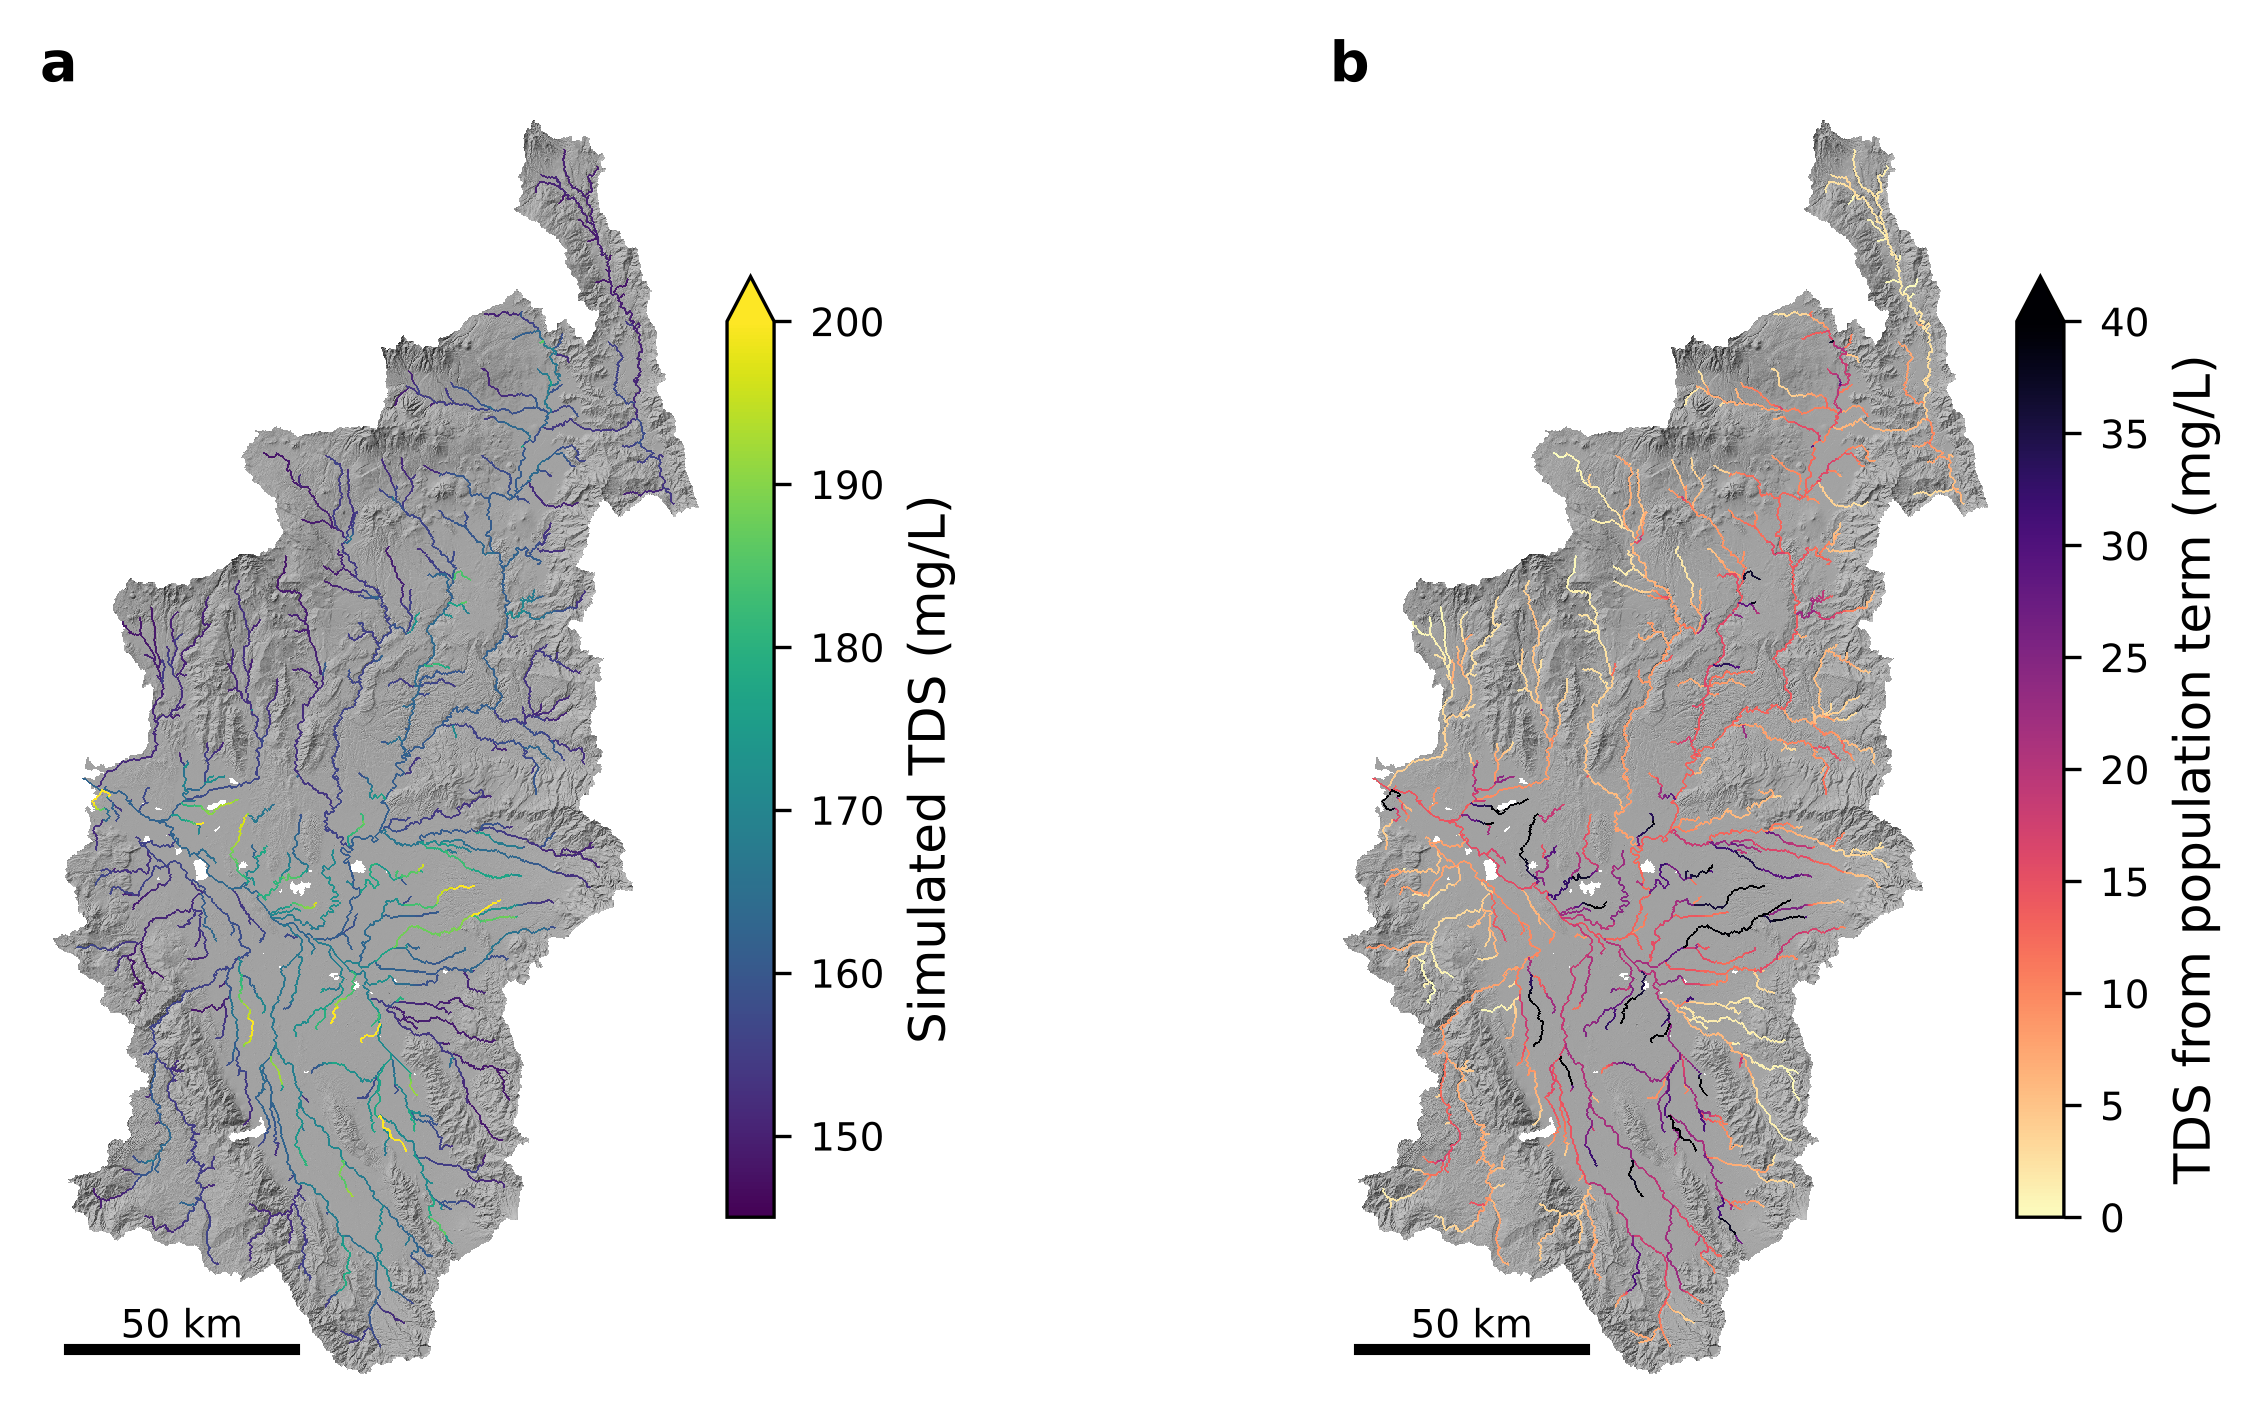
\includegraphics[width=0.92\textwidth]{fig5_simulated_TDS.png}
\caption{(a) TDS simulated by the selected model on channels draining $\geq$20~km$^2$. (b) Part of the simulated TDS attributed to the population term. Background: AW3D30 hillshade.}
\label{fig:map}
\end{figure*}

\begin{figure*}[!t]
\centering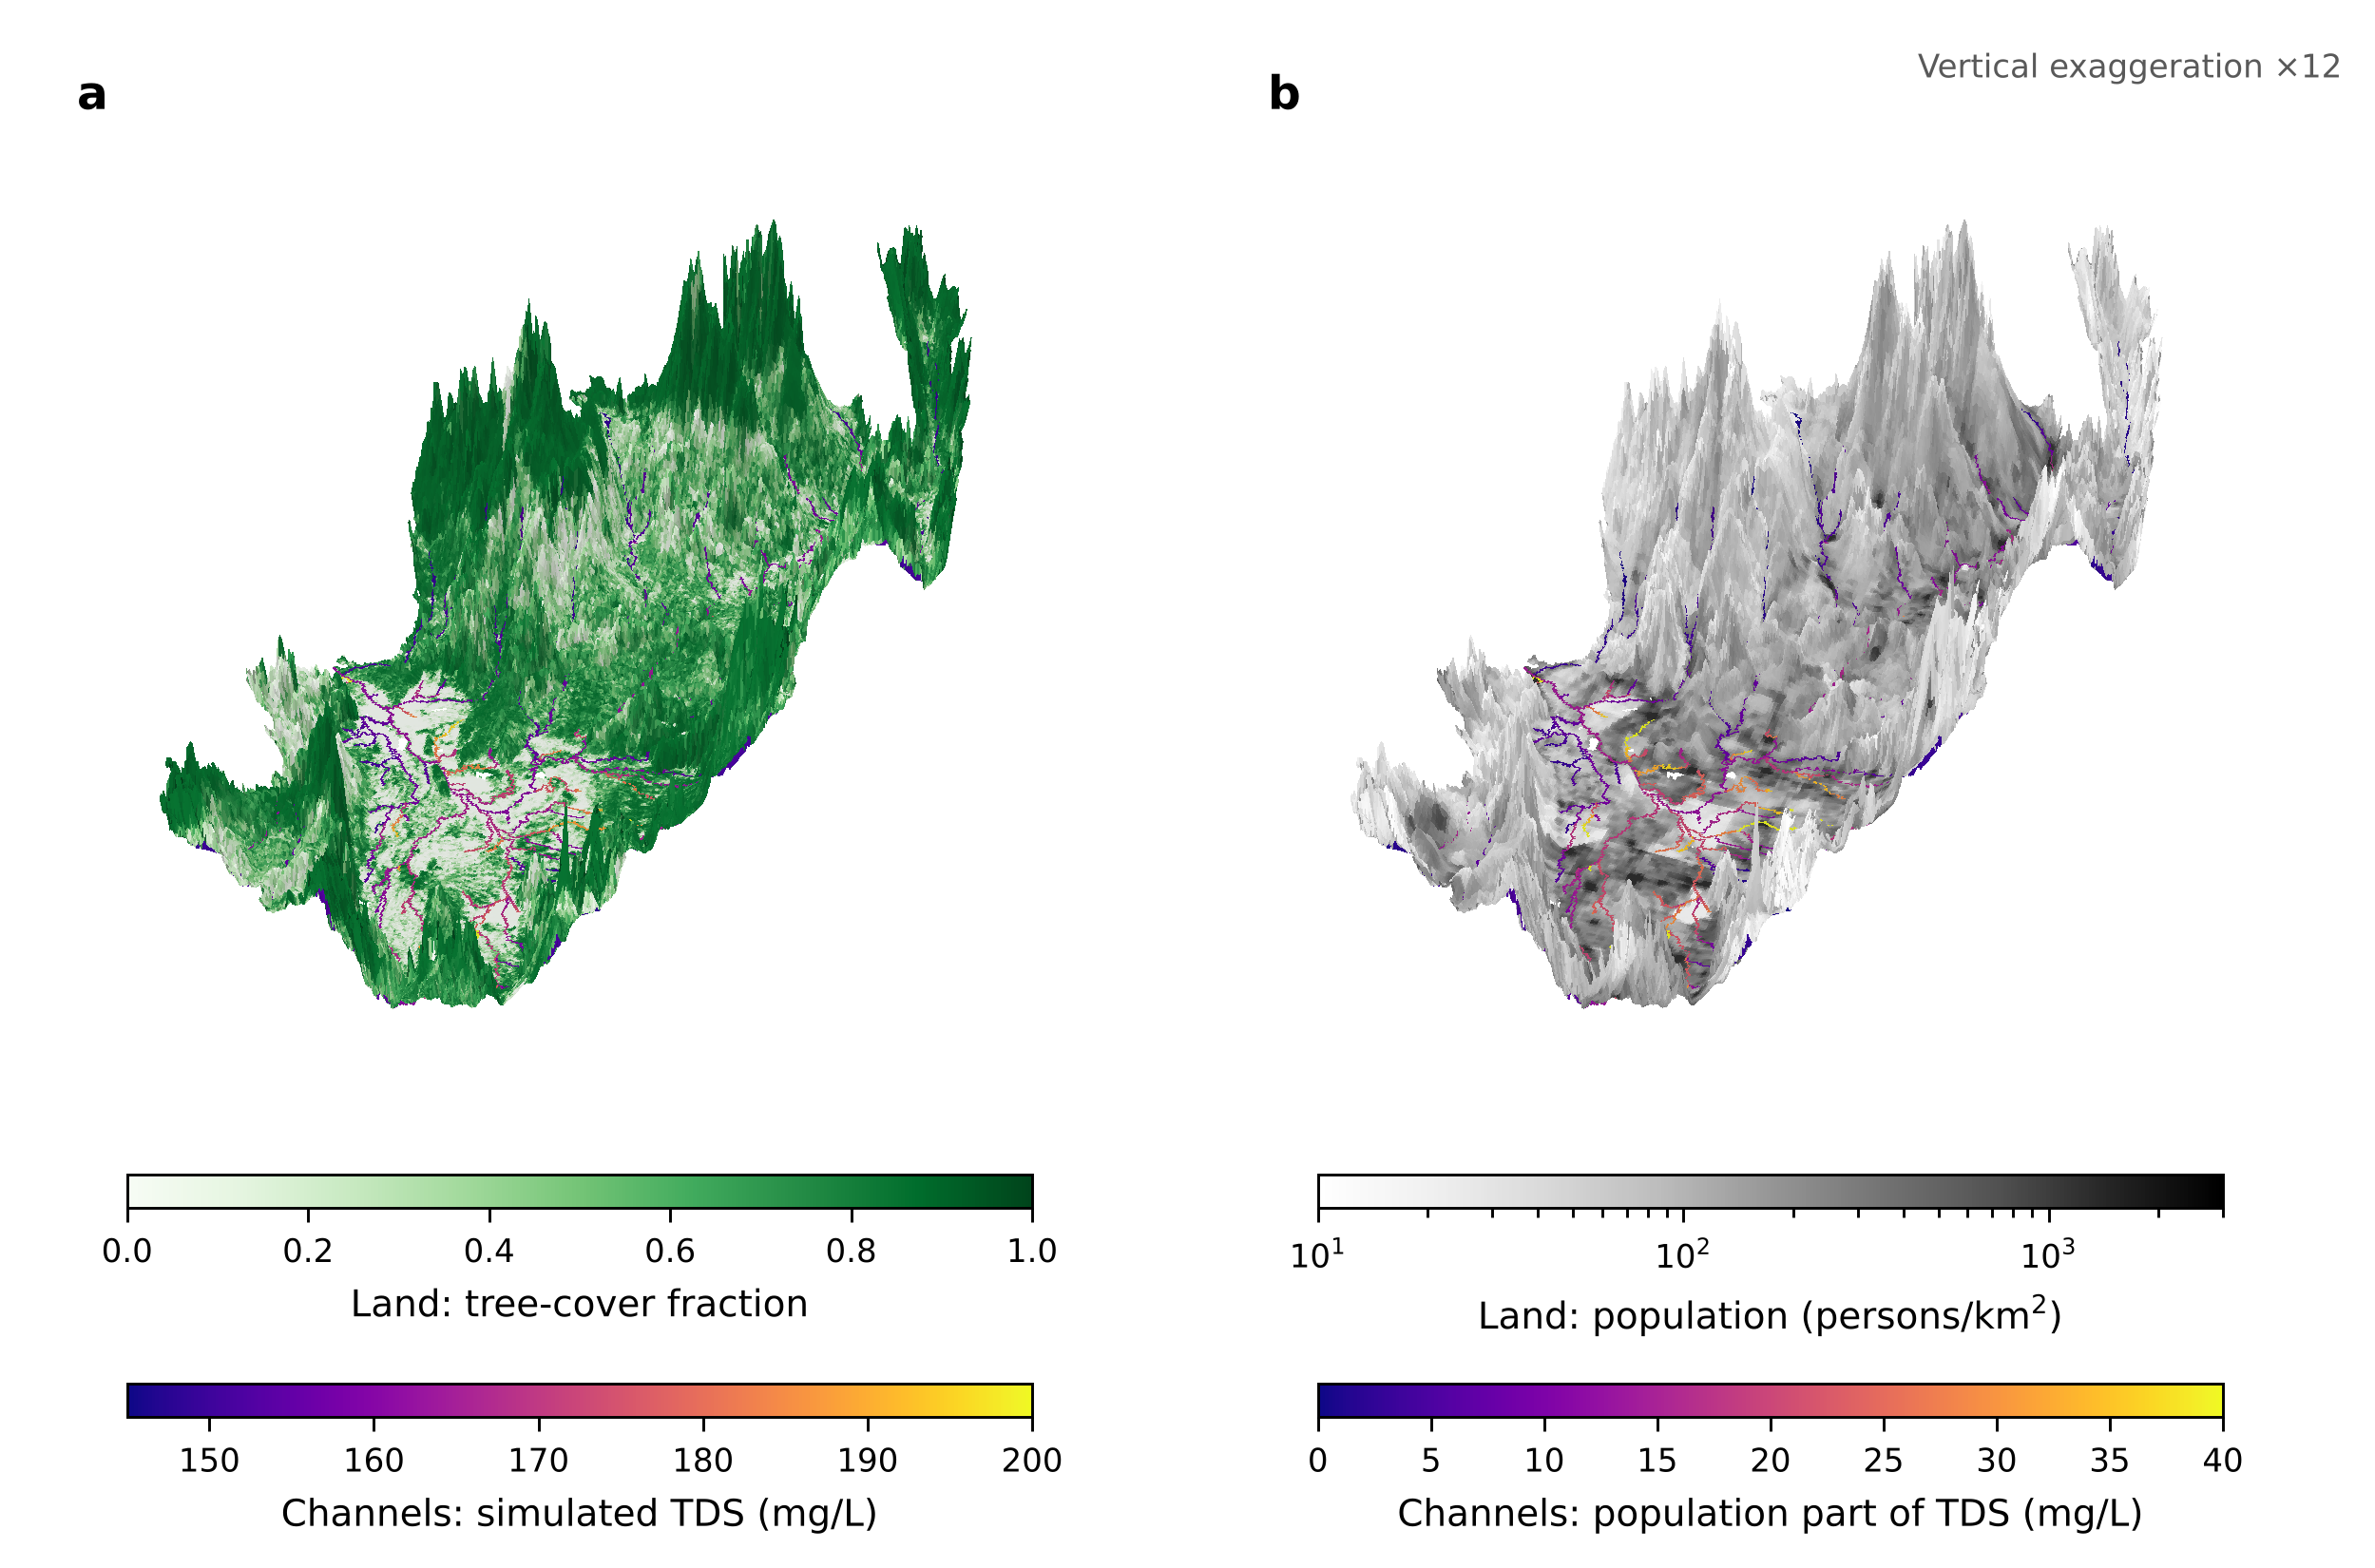
\includegraphics[width=0.94\textwidth]{fig8_3d_terrain_TDS.png}
\caption{3D views of the basin from the south-west (AW3D30 at 450~m, vertical exaggeration $\times$12). (a) Land coloured by tree-cover fraction, with channels draining $\geq$50~km$^2$ coloured by simulated TDS. (b) Land coloured by population density, with channels coloured by the population part of TDS.}
\label{fig:3d}
\end{figure*}

\subsection{How Forests, Farms, Buildings and People Affect Simulated TDS}
Under the selected structure, S4 (population +50\%) raised outlet TDS by 7.3~mg/L (95\% interval 0.0--29.6), and land-cover scenarios changed it by at most 1.0~mg/L (Fig.~\ref{fig:scen}), only through changed runoff. Across all five structures, the population effect was consistently positive (+7.3 to +10.6~mg/L) wherever the fit retained a population term; the five-class fit set it to zero. The land-cover effects were not consistent. Converting 20\% of tree cover to cropland (S1) changed outlet TDS by $-1.0$ to $-23.5$~mg/L, and doubling built-up land (S2) by $-1.0$ to $+17.4$~mg/L. The negative S1 values arise because NNLS assigned cropland a source concentration of zero in the two multi-class structures, so additional cropland runoff dilutes the river---a sign that the fit is not identifying a cropland source, not evidence that farms lower TDS. S3 (cropland to tree cover) gave +0.3 to +5.9~mg/L for the same reason.

\begin{figure*}[!t]
\centering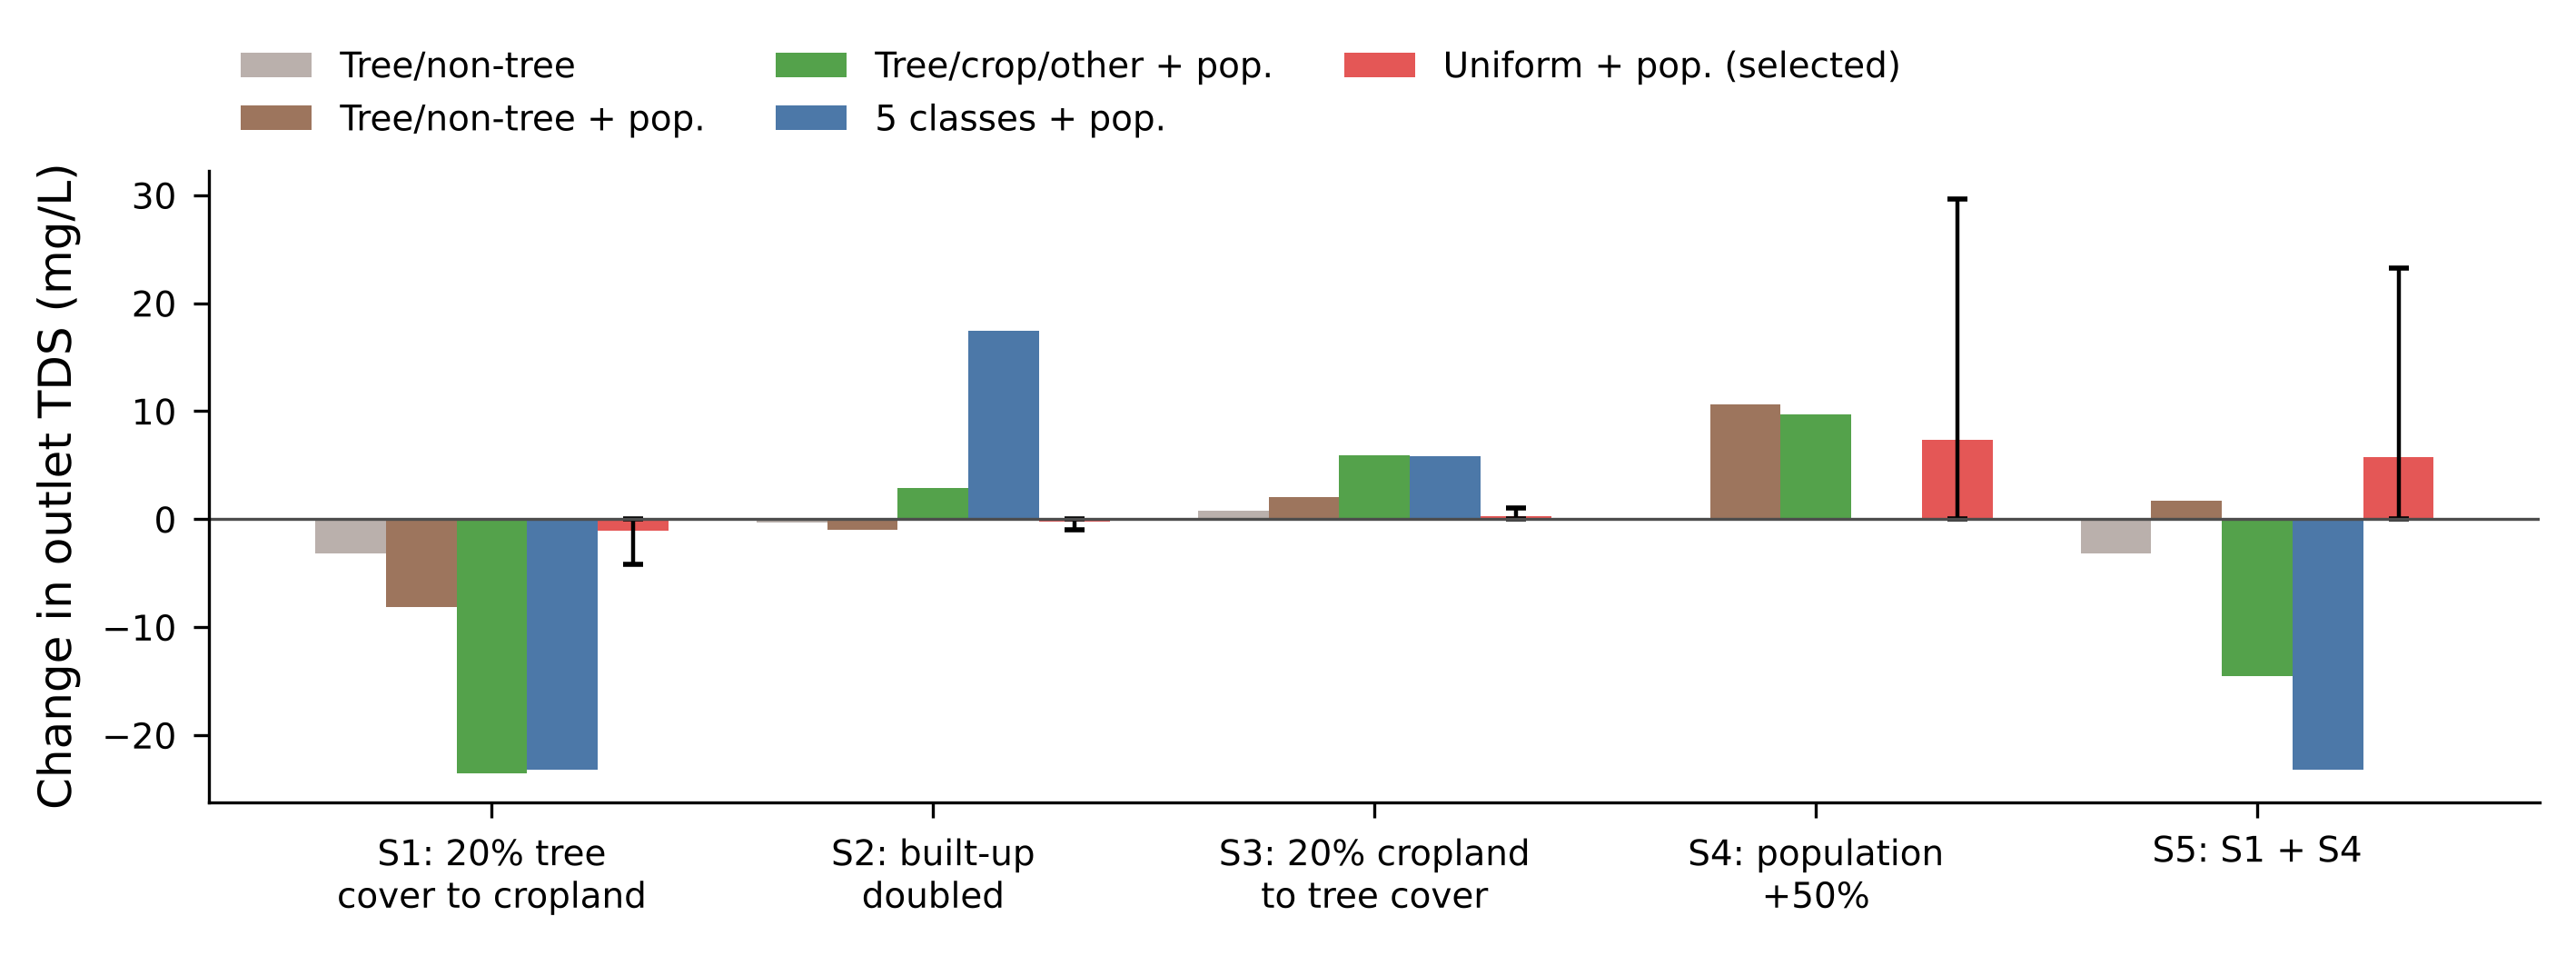
\includegraphics[width=0.9\textwidth]{fig6_land_cover_scenarios.png}
\caption{Change in simulated outlet TDS under scenarios S1--S5 for each model structure, each fitted to the 22 sites. Whiskers on the selected structure are 95\% bootstrap intervals (2000 refits).}
\label{fig:scen}
\end{figure*}

\subsection{Proposed Sampling Network}
The 30 proposed sites (Fig.~\ref{fig:samp}) cover all five tree-cover strata (6 each), small catchments (10--300~km$^2$) where land-cover contrasts are sharpest, and parts of the basin with no published data, including the northern Pulangi headwaters and the eastern uplands.

\begin{figure}[!t]
\centering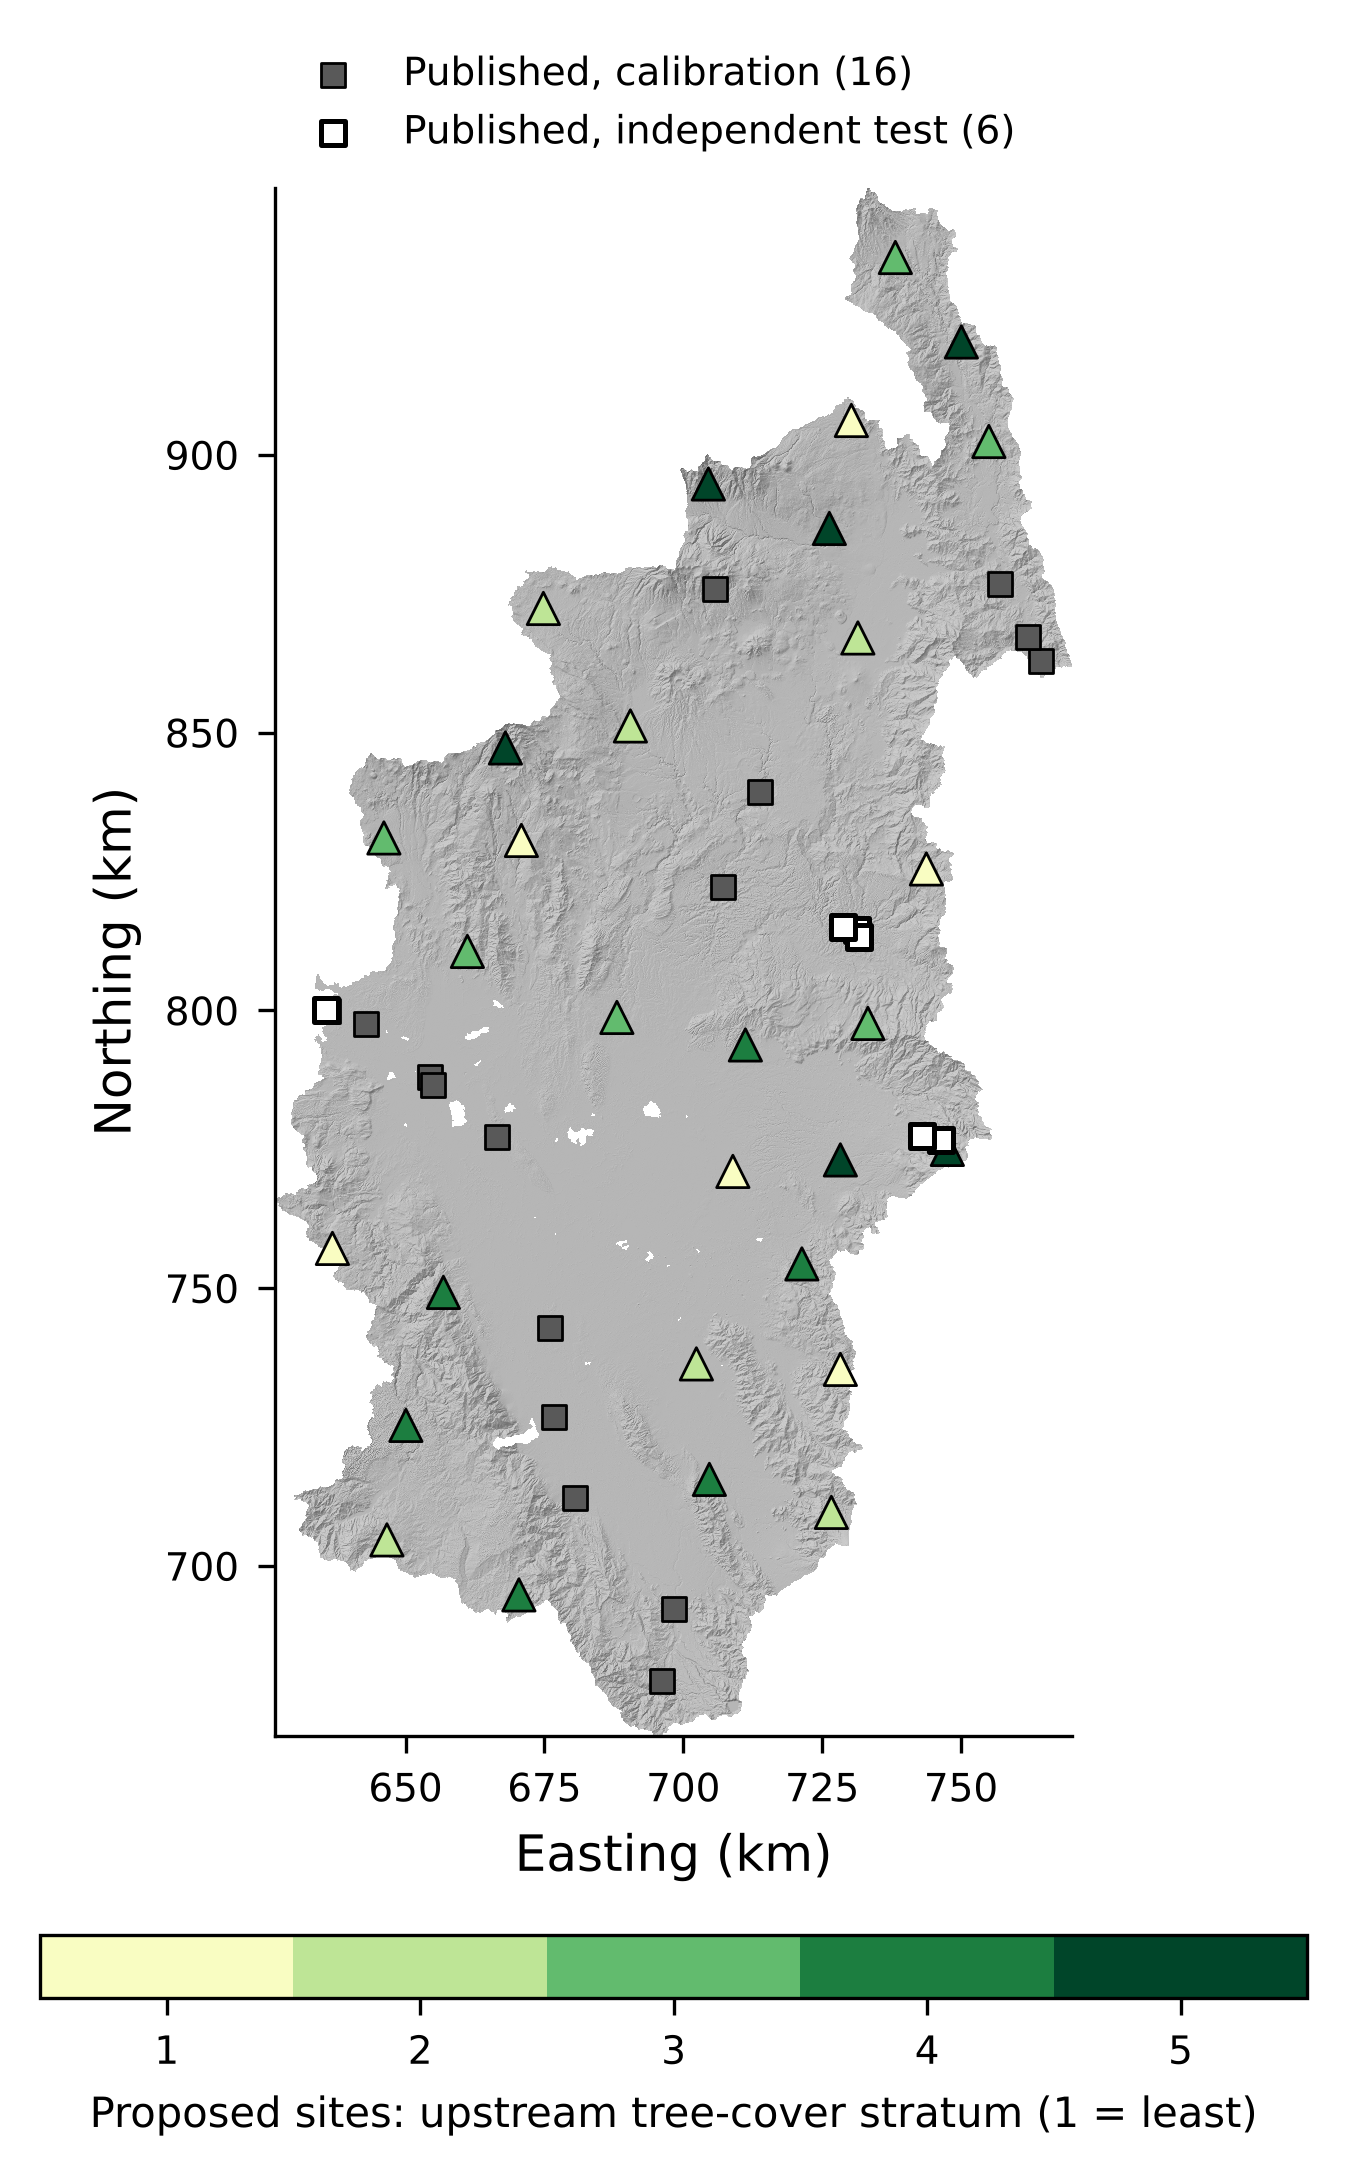
\includegraphics[width=0.92\columnwidth]{fig7_proposed_sampling.png}
\caption{Thirty proposed validation sites (triangles) in five strata of upstream tree-cover fraction, with the 22 published sites (squares).}
\label{fig:samp}
\end{figure}

\section{Discussion}
The main result is negative but useful: with every georeferenced published TDS value we could find, neither land cover nor population predicts TDS across the MRB better than a constant. The first version of this study, on 16 sites, found a tree/non-tree contrast that cross-validated better than the null; 6 independent sites removed it. This is the outcome that validation is meant to detect, and it answers the reviewers' question directly: on present evidence, a weighted overlay of terrain or land-cover factors would encode assumptions that the data do not support.

What the published data do show is that river systems differ more than land cover can explain. The Arakan Valley rivers and the Mt Apo streams carry higher TDS than any land-cover combination in the model predicts, and the Muleta headwaters carry less. Lithology and groundwater inputs are the obvious missing drivers: Mt Apo is a volcano with a geothermal field on its flanks, and solute-rich spring and hydrothermal inflow would raise TDS independently of land use. A geological term (e.g. dominant lithology per catchment from a national geological map) is the most promising addition, but with 7 river systems it would need to be tested on new sites rather than fitted to these. Differences in season, year and method between the sources (2009--2024; probes, meters and laboratory analyses) add further between-river noise; the 52~mg/L gap between the 2022 and 2024 Cotabato City values illustrates it.

The population result is the most robust signal: positive wherever it is retained, physically plausible (domestic wastewater adds dissolved salts) and of a size---about 9\% of outlet TDS---plausible for a basin of 5.16 million people. Its interval nonetheless includes zero, and it should be treated as a hypothesis for the sampling campaign to test.

The model itself is reusable. It is linear in its parameters, runs in seconds on 2.5 million cells, separates water yield from solute sources, and accepts any additional load layer (geology, livestock, mining) as a further column. Its limitations are those of export-coefficient models: steady state, uniform rainfall, conservative TDS, and source concentrations that are fitted rather than measured. The uniform-rainfall assumption matters least for concentrations, since rainfall cancels in Eq.~(\ref{eq:tds}).

\section{Conclusion}
We rebuilt the MRB TDS study on open data with a routed, reproducible model and a validation design that includes an independent test set. Published observations from 22 sites do not support land-cover-based TDS prediction in the basin: no structure beat the training mean, and the simulated effect of forest loss depended on model structure. Population was the only consistently positive driver (+7.3~mg/L for a 50\% increase), but its uncertainty includes zero. Between-river differences, likely geological, dominate the record. The 30-site land-cover-stratified sampling network, with conductivity measured in wet and dry seasons and lithology recorded per catchment, is the next step. All code, inputs, outputs, GeoTIFFs and figures are available at \url{https://github.com/monteropeterdominic-arch/Mindanao-Basin-TDSPM}.

\section*{Acknowledgment}
P.D.C.M. is a scholar of the DOST Science Education Institute. We thank the authors of the published surveys used here, and OpenTopography, ESA, WorldPop and the OpenStreetMap contributors for open data.

\footnotesize
\balance
\begin{thebibliography}{99}
\bibitem{asnake} K. Asnake, H. Worku, and M. Argaw, ``Assessing the impact of watershed land use on Kebena river water quality in Addis Ababa, Ethiopia,'' \textit{Environ. Syst. Res.}, vol.~10, art.~3, 2021, doi: 10.1186/s40068-020-00208-y.
\bibitem{merriam} E. R. Merriam, M. P. Strager, and J. T. Petty, ``Source water vulnerability to elevated total dissolved solids within a mixed-use Appalachian River basin,'' \textit{PLoS Water}, vol.~1, art.~e0000035, 2022, doi: 10.1371/journal.pwat.0000035.
\bibitem{stephens} M. J. Stephens \textit{et al.}, ``A joint Gaussian process model of geochemistry, geophysics, and temperature for groundwater TDS in the San Ardo Oil Field, California, USA,'' \textit{J. Hydrol.}, vol.~661, art.~133540, 2025, doi: 10.1016/j.jhydrol.2025.133540.
\bibitem{aju} C. D. Aju \textit{et al.}, ``Is TDS enough for ion-specific groundwater quality screening? A geospatial machine learning assessment,'' \textit{Appl. Geochem.}, vol.~203, art.~106803, 2026, doi: 10.1016/j.apgeochem.2026.106803.
\bibitem{malcz} J. Malczewski, ``GIS-based multicriteria decision analysis: A survey of the literature,'' \textit{Int. J. Geogr. Inf. Sci.}, vol.~20, no.~7, pp.~703--726, 2006.
\bibitem{chen} Y. Chen, J. Yu, and S. Khan, ``Spatial sensitivity analysis of multi-criteria weights in GIS-based land suitability evaluation,'' \textit{Environ. Model. Softw.}, vol.~25, no.~12, pp.~1582--1591, 2010.
\bibitem{ligmann} A. Ligmann-Zielinska, P. Jankowski, A. Najwer, and Z. Zwoli\'nski, ``A streamlined approach to uncertainty and sensitivity analysis for models with spatial outputs,'' \textit{Int. J. Geogr. Inf. Sci.}, vol.~38, pp.~1531--1554, 2024.
\bibitem{johnes} P. J. Johnes, ``Evaluation and management of the impact of land use change on the nitrogen and phosphorus load delivered to surface waters: The export coefficient modelling approach,'' \textit{J. Hydrol.}, vol.~183, pp.~323--349, 1996.
\bibitem{sparrow} R. A. Smith, G. E. Schwarz, and R. B. Alexander, ``Regional interpretation of water-quality monitoring data,'' \textit{Water Resour. Res.}, vol.~33, no.~12, pp.~2781--2798, 1997.
\bibitem{tu} J. Tu, ``Spatially varying relationships between land use and water quality across an urbanization gradient explored by geographically weighted regression,'' \textit{Appl. Geogr.}, vol.~31, pp.~376--392, 2011.
\bibitem{guiamel} I. A. Guiamel and H. S. Lee, ``Watershed modelling of the Mindanao River Basin in the Philippines using the SWAT for water resource management,'' \textit{Civ. Eng. J.}, vol.~6, no.~4, pp.~626--648, 2020.
\bibitem{tadono} T. Tadono, H. Ishida, F. Oda, S. Naito, K. Minakawa, and H. Iwamoto, ``Precise global DEM generation by ALOS PRISM,'' \textit{ISPRS Ann. Photogramm. Remote Sens. Spatial Inf. Sci.}, vol.~II-4, pp.~71--76, 2014.
\bibitem{zanaga} D. Zanaga \textit{et al.}, ``ESA WorldCover 10 m 2021 v200,'' Zenodo, 2022, doi: 10.5281/zenodo.7254221.
\bibitem{worldpop} A. J. Tatem, ``WorldPop, open data for spatial demography,'' \textit{Sci. Data}, vol.~4, art.~170004, 2017, doi: 10.1038/sdata.2017.4.
\bibitem{wang} L. Wang and H. Liu, ``An efficient method for identifying and filling surface depressions in digital elevation models for hydrologic analysis and modelling,'' \textit{Int. J. Geogr. Inf. Sci.}, vol.~20, no.~2, pp.~193--213, 2006.
\bibitem{ocallaghan} J. F. O'Callaghan and D. M. Mark, ``The extraction of drainage networks from digital elevation data,'' \textit{Comput. Vis. Graph. Image Process.}, vol.~28, pp.~323--344, 1984.
\bibitem{brillantes} E. L. Brillantes \textit{et al.}, ``Water quality status of the Allah River highlights emerging conservation concerns in a partially protected landscape of the southern Philippines,'' Research Square preprint rs-10460022, v1, 2026.
\bibitem{dimalen} F. K. Dimalen \textit{et al.}, ``Rapid assessment of water quality in Rio Grande de Mindanao, Philippines,'' \textit{AACL Bioflux}, vol.~18, no.~6, pp.~2749--2760, 2025.
\bibitem{dumago} S. W. L. Dumago, G. R. Puno, and S. S. Ingotan, ``Water quality assessment in various land use and land cover of Muleta Watershed, Bukidnon, Philippines,'' \textit{J. Biodiv. Environ. Sci.}, vol.~12, pp.~201--209, 2018.
\bibitem{galarpe} V. R. K. R. Galarpe, K. J. L. Heyasa, and B. B. L. Heyasa, ``Water quality and risk assessment of tributary rivers in San Fernando, Bukidnon, Philippines,'' \textit{J. Biodiv. Environ. Sci.}, vol.~11, pp.~266--273, 2017.
\bibitem{villabeto} S. C. Villabeto and L. Simpol, ``Monitoring and baseline profile confluence of Kulaman and Tinanan rivers in Arakan Valley Philippines,'' \textit{Sch. Acad. J. Biosci.}, vol.~2, no.~2, pp.~90--96, 2014.
\bibitem{quimpang} V. T. Quimpang \textit{et al.}, ``Fish abundance and physico-chemical properties of Matingao River and Marbel River, Mount Apo Natural Park, Mindanao, Philippines,'' \textit{CMU J. Sci.}, vol.~23, no.~2, pp.~14--19, 2019, doi: 10.52751/drfa8273.
\bibitem{alombro} N. C. Alombro, R. C. Guiamadil, W. U. Datumama, and J. P. A. Catipay, ``Evaluation of organic pollution using algal diversity in rivers of Cotabato City, Bangsamoro Autonomous Region in Muslim Mindanao (BARMM), Mindanao Island, Philippines,'' \textit{Nature Environ. Pollut. Technol.}, vol.~22, no.~4, 2023.
\bibitem{chow} V. T. Chow, D. R. Maidment, and L. W. Mays, \textit{Applied Hydrology}. New York, NY, USA: McGraw-Hill, 1988.
\bibitem{lawson} C. L. Lawson and R. J. Hanson, \textit{Solving Least Squares Problems}. Englewood Cliffs, NJ, USA: Prentice-Hall, 1974.
\bibitem{roberts} D. R. Roberts \textit{et al.}, ``Cross-validation strategies for data with temporal, spatial, hierarchical, or phylogenetic structure,'' \textit{Ecography}, vol.~40, pp.~913--929, 2017.
\bibitem{efron} B. Efron and R. J. Tibshirani, \textit{An Introduction to the Bootstrap}. New York, NY, USA: Chapman \& Hall, 1993.
\end{thebibliography}
\end{document}
